\begin{frame}{Signal Protocol}
    \framesubtitle{Il protocollo: Double Ratchet}

    Algoritmo utilizzato per il proseguimento della conversazione, dopo averla inizializzata tramite X3DH.\newline\pause
    \cite{doubleratchet}, \cite{VanDam} \newline   
    A differenza di X3DH usa una catena KDF, come mostrato in figura \ref{tag: KDF chain}.

    \begin{figure}
        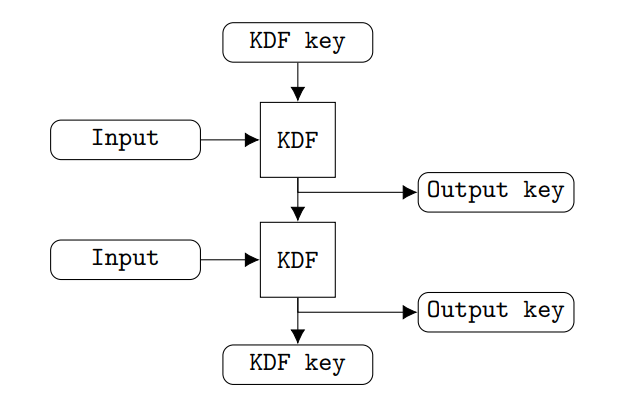
\includegraphics[width=.5\textwidth]{KDF chain.png}
        \caption{Catena KDF}
        \label{tag: KDF chain}
    \end{figure}

    \note{
        La catena KDF usa l'output di una KDF come input per un'altra applicazione della KDF.\newline
        Ogni \textit{output key} può essere utilizzata per cifrare un messaggio.\newline
        Tale catena garantisce:
        \begin{itemize}
            \item Resilienza: l'output appare randomico
            \item Forward secrecy: garantita dalla non-invertibilità della KDF
            \item Future secrecy: garantita se l'input della KDF \(i+1\) non è il solo output della KDF \(i\). Per garantire ciò è necessario usare un \textbf{DH ratchet}
        \end{itemize}

    }
\end{frame}

\begin{frame}{Signal Protocol}
    \framesubtitle{Il protocollo: Double Ratchet}
    Combinando una catena KDF con un DH ratchet otteniamo un algoritmo Double ratchet che garantisce sia \textit{forward secrecy} che \textit{future secrecy}. \newline\pause
    DH ratchet infatti modifica gli input delle KDF in modo tale che, se anche una chiave venisse compromessa, si sia in grado di ristabilire la segretezza dall'applicazione successiva di una KDF.\newline
\end{frame}

\begin{frame}{Signal Protocol}
    \framesubtitle{Il protocollo: Double Ratchet}
    Sia Alice che Bob hanno tre catene KDF da utilizzare:
    \begin{itemize}
        \item DH ratchet
        \item Sending ratchet
        \item Receiving ratchet
    \end{itemize}\pause
    Ogni volta che Alice vuole inviare un messaggio a Bob aggiornerà la catena \textit{sending ratchet} producendo una nuova chiave di output e invierà a Bob il proprio messaggio cifrato con essa.
\end{frame}

\begin{frame}{Signal Protocol}
    \framesubtitle{Il protocollo: Double Ratchet}
    La catena di invio di Alice deve essere sincronizzata con quella di ricezione di Bob e viceversa e devono iniziare nella stessa posizione (caratteristica garantita da X3DH applicato prima del Double ratchet).\newline\pause
    In queste condizioni tuttavia non è ancora garantita la \textit{future secrecy}
\end{frame}

\begin{frame}{Signal Protocol}
    \framesubtitle{Il protocollo: Double Ratchet}
    Per garantire \textit{future secrecy} Bob invierà come parte di uno dei suoi messaggi una nuova chiave pubblica Diffie-Hellman.\pause\newline
    Alice userà questa chiave per far avanzare la catena DH-ratchet, imponendo così il reset delle catene di ricezione e invio. In parallelo anche la catena DH-ratchet di Bob verrà aggiornata.\newline\pause
    Un comportamento analogo verrà applicato da Bob sulle proprie catene.\newline\pause
    Questo scambio di chiavi DH può avvenire ogniqualvolta necessario ma normalmente avviene a ogni messaggio scambiato.
    \cite{doubleratchetVid}

    \note{
        Questo sistema di catene garantisce dunque:
        \begin{itemize}
            \item Forward security: grazie alle catene di invio e ricezione, caratterizzate da funzioni non invertibili, non è possibile retrocedere ai messaggi inviati in precedenza
            \item Future secrecy: grazie alla catena DH-ratchet se anche si riesce a intercettare un messaggio e decrittarlo si resettano le catene di invio e ricezione, rendendo impossibile generare in anticipo le chiavi che verranno utilizzate in futuro
            \item Funzionamento asincrono: se Alice invia dieci messaggi a Bob e lui non risponde man mano, egli comunque sarà in grado di ricostruire la sequenza di chiavi utilizzata da Alice e dunque leggere i messaggi
            \item In ogni messaggio viene indicato il numero di messaggi già inviati sulla stessa catena quindi se un messaggio va perso si può o aspettarne l'arrivo o far avanzare la catena di tante posizioni quanti messaggi sono andati persi.
        \end{itemize}

        N.B. Le chiavi vengono eliminate non appena utilizzate per decifrare un messaggio, se delle chiavi non vengono utilizzate vengono conservate finché non arriverà il messaggio corrispondente.
    }
\end{frame}

\begin{frame}{Signal Protocol}
    \framesubtitle{Il protocollo: Double Ratchet}

    \begin{figure}
        \centering
        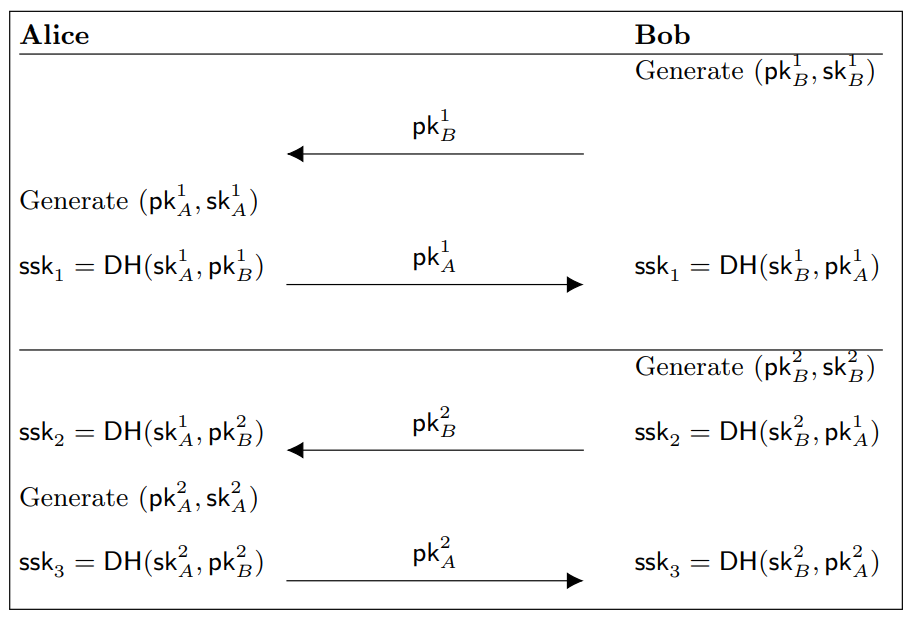
\includegraphics[width=.6\textwidth]{dh ratchet.png}
        \caption{DH ratchet}
        \label{tag: DH ratchet}
    \end{figure}

\end{frame}